\documentclass[../main.tex]{subfiles}
\graphicspath{{\subfix{../../images/}}}
\begin{document}

\chapter{Background \& Prior Work}\label{chap:bg_theory}

\begin{quote}
  \emph{Even a simple movement is a global body event.}
  \raggedleft{--- Bizzi \& Ajemian, \emph{2020}}
\end{quote}  


% \begin{quote}
%   \emph{We have some idea as to the intricate design of the puppet and the puppet strings, but we lack insight into the mind of the puppeteer.}
%   \raggedleft{--- Emilio Bizzi \& Ajemian \emph2020}}
% \end{quote}



Ideas from theory we can keep in mind for our experiment that we can look out for in interpreting our results:
- Do subjects display model-based or model-free learning, what would distringuish these two possibilities?
- Are subjects creating new, bespoke ``controllers'' for this task or are they adapting from existing movement repertoire?
- Cost functions, optimization
- System identification (control), policy optimization


% Implicit / Explicit 
% Model-based / Model-free 
% Slow / Fast
- Krakauer et al.'s motor learning review categorization of motor learning places prior work into the following classes: - Adaptation - Sequence Learning - De Novo Learning - Motor Acuity - Expertise. Align our interest and work into these categories and discuss how we're thinking about this...

- The mininum intervention principle, Scholz and Schoner

The UCM is not a hard-and-fast principle, as nothing is in the motor system. Rather, as we've seen elsewhere, there seems to be a spectrum of control. This could be explained through a composite cost function which penalizes deviations from prior movement strategies[@raczSpatiotemporalAnalysisReveals2013]. There is much research pushing back on optimal control, uncontrolled manifold hypothesis, and this will be addressed in {+@sec:experiment}. 


- Optimal feedback control as an algorithm which generate minimally intervening motor actions

- Motor control is distributed throughout the brain\cite{sejnowskiPerspectivesCognitiveNeuroscience1988}.

- From physiology, we can see that the motor system is highly distributed and constructs action based on a variety of state dependence. The theoretical question becomes \emph{when does it make computational sense to construct action by composing control policies rather than selecting or tuning a single policy?} When is policy arbitration computationally advantageous?

- A policy is a function of your ``state'' where the output is motor actions, decisions about which muscles to activate. Policies can be formalized as a probability distribution over actions, and can be parameterized in a number of ways, from simple distributions to dynamical systems, to neural networks.

- We can speculate that practice and expertise as convincing your brain to commit to a more complex policy (or maintain commitment to a current level of complexity).

- Certain movement disorders can be viewed as involving information bottlenecks -- communicating the policy given your current state[@gershmanRewardcomplexityTradeoffSchizophrenia2020] 
- "optimal compression means knowing the state probabilities" having some form of a model -- marginal state distribution (mean state occupancies?) SR row sums?
- "the memory demand of policies acts as an information bottleneck in action selection"

- "Default policy" as habits \cite{pirayLinearReinforcementLearning2019}

- Our theory of neural control of the hand is approximately: control is composed of a number of overlapping cortical controllers. 

These receive input from goal-oriented centers as well as a plethora of ongoing contextual, perceptual information. 

Control is modulated by these inputs, adjusting “online” to disturbances. 

Cortical controllers are massively redundant; the contain all available information about the context of an ongoing task, branching to an array of downstream spinal centers as well as converging to individual spinal innervations. 

Our hypothesis is that subjects will use their vast repertoire of pre-existing control schemes/movements/controllers/patterns/activations until they find a pattern that increases their success, upon which they will “hone” this scheme by refining the discovered movement. 

This hypothesis predicts an exploratory, or “search”, period of the task, followed by (or overlapping with) an exploitative or “honing” period as subjects settle on a motor solution. 




Models of Adaptation
- two-rate models \cite{smithInteractingAdaptiveProcesses2006}
- linear dynamical system for adaptation \cite{chengModelingSensorimotorLearning}


- Optimal feedback control, now introduced to motor control field 25 years ago, remains the best (most elegant) explanation we have for motor coordination, but there's no adaptation or learning.

The control setup writes a cost, environment has some dynamics.




\section{Physiology of Hand Control}

%  In this section, we support the claim that the motor system's organizing principle is redundancy at all levels, and that this redundancy supplies us with flexibility. This flexibility is illustrated in the CNS's demonstrated hierarchy in both planning and execution of action. 

%  - what can physiology tell us about the movement problem?
%   - can it inform theory to describe motor solutions?
%   - this will inform the shape our models
%   - the constraints of our tasks, questions
  
% - what do we know about brain and motor?
%   - hands, thumbs, forearms anatomy
%   - synergies, cm connections
%     - bizzi
%     - porter & lemon
%     - from muscles to cortex
%     - 
% - loops and controllers
%   - graziano
%   - cerebellum
%   - cortex, hantman
%   - mouse, primate
%   - basal ganglia 

As we hope to make progress engineering naturalistic artificial movement, it will be beneficial to review what is known about the biological movement system. Beginning with the architecture of the motor system and it's relation to dexterity will provide a scaffold on which we can hang our experimental and theoretical investigations detailed in {+@sec:experiment} and {+@sec:theory}. Specifically, we can use results from prior physiological investigations to ground our perspective on the computations relevant to skilled hand movements. We find that the dexterous solutions produced by the human motor system rely on a incredibly complex architecture, but one in which a spectrum of modularity and redundancy appear to be organizing principles. 

Muscles are composed of fibers which contract due to chemical gradients produced at the neuromuscular junction by action potentials emanating from alpha-motoneurons (AMN) in the ventral horn of the spinal cord. The quantum of motor output is the motor unit (MU), defined as a single motoneuron axon and the set of junctions its axon branches form with one or more muscle fibers. The innervation ratio of a particular muscle unit is the number of junctions it innervates. In muscles of the arm, the number of MUs and their innervation ratios each range from tens to hundreds per muscle and per motor unit, respectively, decreasing as muscles become more distal. 


Paradoxically, however, the well-known signal-dependent noise in models of motor output has been found to be higher for hand muscles than for more proximal muscles, likely due to small numbers of motor units compare to larger muscles[@harrisSignaldependentNoiseDetermines1998;@fuglevandMechanicalPropertiesNeural2011]. 

Muscle fibers are contained within muscle compartments, and each muscle may have one or more compartments. The fingers of the hand are extended by the extensor digitorum (ED) which contains four compartments, one for each of the tendons the muscle produces. Each tendon connects to the three metaphalangeal joints of each digit. The fingers are flexed by two muscles, the flexor digitorum superficialis (FDS) and the flexor digitorum profundus (FDP). Like the ED, these muscles produce four tendons, one to each finger from each of their four compartments. As such, one must coactivate these agonist and antagonist muscles in order to extend or flex a single finger in isolation[@fuglevandMechanicalPropertiesNeural2011]. Adduction and abduction of the fingers is produced by the 19 intrinsic muscles of the hand, each of which has their origin and insertion points within the hand itself[@vanduinenConstraintsControlHuman2011]. The intrinsic muscle tendons form a kind of network around each of the digits. The human hand, thumb, and forearm system contains more than 30 muscles and at least 20 degrees of freedom are theoretically available for actuation. However, due to biomechanical coupling, the effective degrees of freedom is presumably less than 20.

One study found that tendons of the fingers are arranged in such a way as to perform a kind of anatomical computation which expands the mechanical capabilities of the appendage by sharing force across its tendon network[@Valero-Cuevas2007]. Such computations embedded in the musculoskeletal structure are additional complexity when theorizing about neural control of the hand. 


These redundancies at the neurophysiological level play a role in "spillover", where contractions of one muscle or muscle compartment seem to spill over into neighboring muscles and muscle compartments. This is evident in the difficulty of moving single fingers individually. As mentioned previously, this may be a hardwired constraint or a byproduct of plasticity induced by behavioral requirements. 

> Spillover has been shown in experiments studying the ‘recruitment thresholds’ (defined below) of motor units ac ting on other digits during single digit contractions (Kilbreath & Gandevia, 1994; Butler et al. 2005; van Duinen et al. 2009). In these experiments, motor units were recorded from one (test) compartment of the respective muscles, while subjects were asked to contract the compartment of the other digits up to 50\% of their maximal force. When the subjects contracted these other digits (one by one), motor units of the test compartment were often recruited. The amount of force produced by the other digits at the time of recruitment of the motor unit of the test compartment is termed the recruitment threshold. The general finding for all three muscles was that, the closer the contracting compartment to the test finger, the more motor units were recruited. [...] One has to ask whether this spillover is functional. Is the frequent recruitment of motor units ac ting on the little finger when we extend the thumb part of a fixed pattern of muscle activation, perhaps to balance forces around the wrist? (Duinen & Gandevia 2011) 

























\section{Motor Units to Muscles}\label{motor-units-to-muscles}

The quantum of motor output is the motor unit (MU), defined as a single motoneuron axon and the set of junctions the terminals of its axon branches form with one or more muscle fibers. The MU provides the motor system with spatial redundancy at the muscle level: multiple muscle fibers contract due to a single alpha motoneuron (AMN) spike in the spinal cord's ventral horn, and multiple AMNs may overlap in their innervations. The forces produced by motor units span several orders of magnitude, though most units produce very small forces. Here we find temporal redundancy: in order to produce movements, MUs combine to generate a range of forces{[}@fuglevandMechanicalPropertiesNeural2011{]}. Since the innervation ratios of muscles in the forearm and hand are relatively small compared to more proximal muscles (which contain thousands of MUs), the logarithmic recruitment and redundancy of motor units enables the hand to produce movements with very fine spatiotemporal resolution.

Muscle fibers are contained within muscle compartments, and each muscle may have one or more compartments. The fingers of the hand are extended by the extensor digitorum (ED) which contains four compartments, one for each of the tendons the muscle produces. Each tendon connects to the three metaphalangeal joints of each digit. The fingers are flexed by two muscles, the flexor digitorum superficialis (FDS) and the flexor digitorum profundus (FDP). Like the ED, these muscles produce four tendons, one to each finger from each of their four compartments. As such, one must coactivate these agonist and antagonist muscles in order to extend or flex a single finger in isolation{[}@fuglevandMechanicalPropertiesNeural2011{]}. Adduction and abduction of the fingers is produced by the 19 intrinsic muscles of the hand, each of which has their origin and insertion points within the hand itself{[}@vanduinenConstraintsControlHuman2011{]}. The intrinsic muscle tendons form a kind of network around each of the digits. The human hand, thumb, and forearm system contains more than 30 muscles and at least 20 degrees of freedom are theoretically available for actuation. However, due to biomechanical coupling, the effective degrees of freedom is presumably less than 20.

This structure exists in order to facilitate the acquisition of new skills and the generalization of existing skills to new contexts. While the anatomy of the hand and forearm presents constraints on movement, the system remains capable of producing an incredible variety of movement patterns{[}@yanUnexpectedComplexityEveryday2020;@Basmajian1963{]}\footnote{In   a classic study, Basmajian and colleagues showed that it is possible   to activate single motor units in the thumb abductor.}. The structure of the neuromuscular system that underlies this variety offers many clues as to the relevant computations required for dexterous movement. In \{+@fig:low\_variance\_PCs\}, Yan et al.~show how even low-variance principle components of joint kinematics during object grasping and ASL signing display correlational structure and not merely noise. That is, the production of hand movement is highly task-specific, where individual tasks are linked to bespoke muscle activations patterns.

\begin{figure}[H]
\centering
  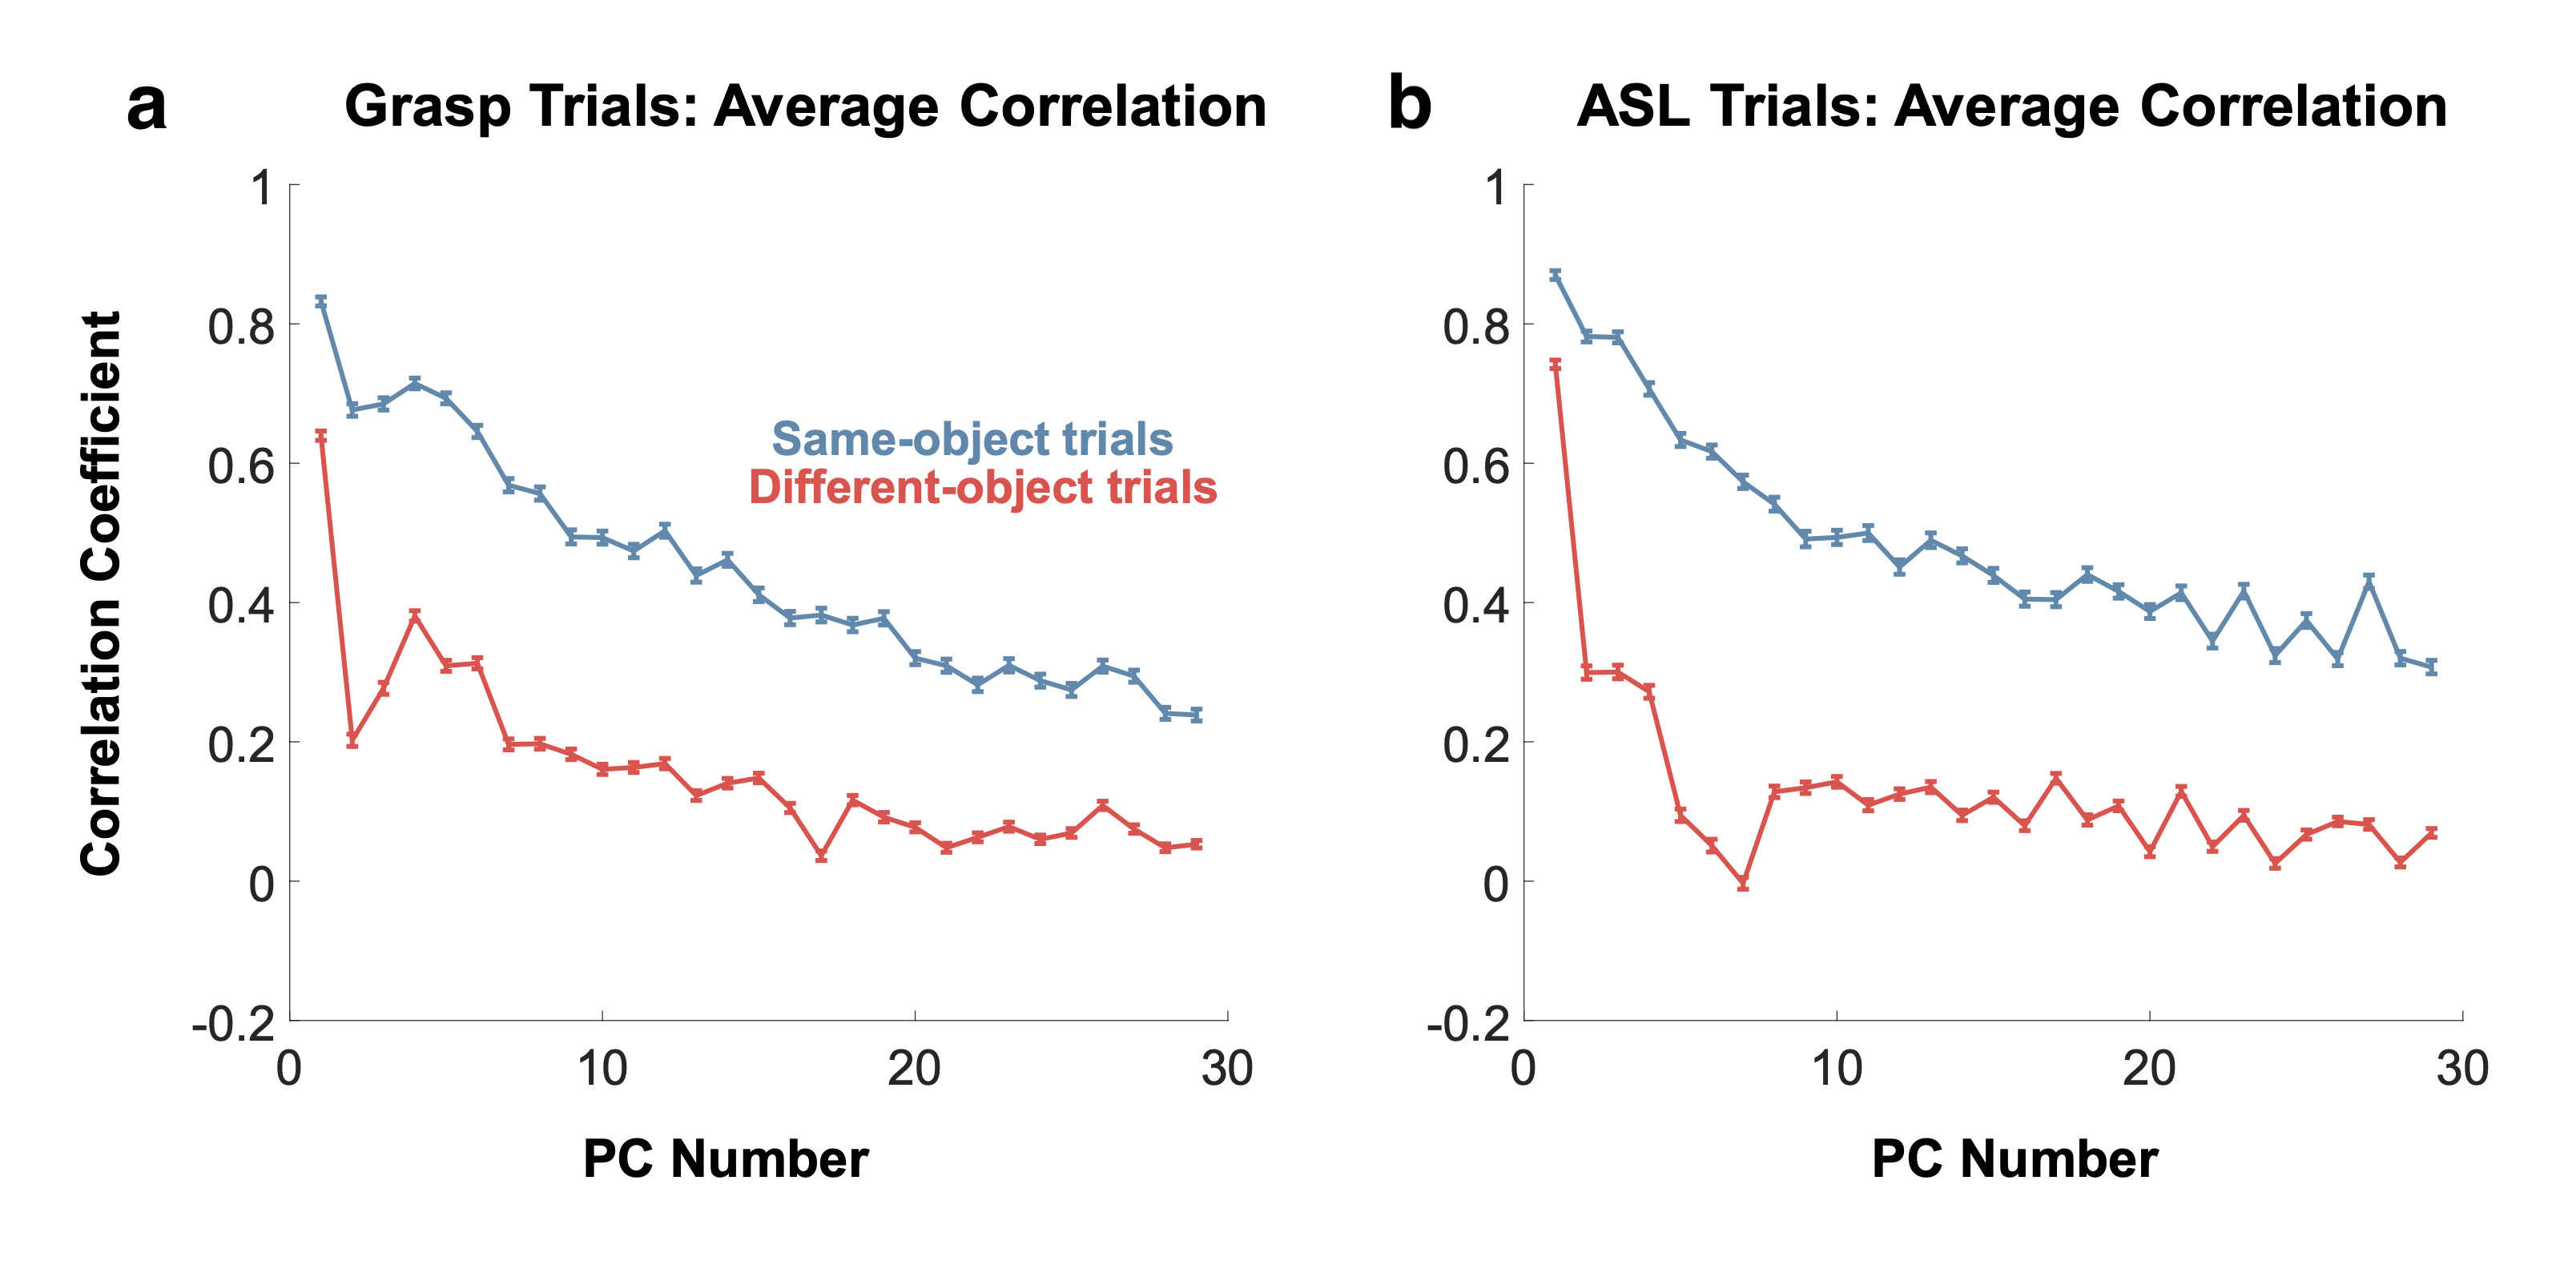
\includegraphics[width=1.0\textwidth]{background_theory/low_variance_PCs.png}
  \caption[Low-variance PCs contain task-relevant information]{Taken from Yan et al.~2020. Plots show mean correlations between hand joint kinematic trajectories during grasp trials with the same (blue) and different (red) objects (a) and ASL signs (b) projected onto the same principle components. Correlations are averaged across 8 subjects. Within-object and within-sign correlations are systematically higher than their shuffled counterparts. Error bars denote SEM. This data supports the idea that low-variance components of kinematics data contain task-specific structure rather than merely reflecting noise. This is encouraging for our experiments, which hope to extend this idea into careful analyses of task specific features of EMG data across learning and in response to perturbations.}\label{fig:low_variance_PCs}
\end{figure}













\subsection{Coordinative Structures}\label{coordinative-structures}

Many studies have contributed to the concept of synergies as a hard-wired organizing feature of the motor system{[}@mussa-ivaldiMotorLearningCombination2000,@DAvella2003{]}. However, these works tend to extrapolate from non-primate preparations, particularly in the frog, and use tasks which are inherently low-dimensional to explain covariance structure in primate and human kinematic and electromyography data{[}@giszterMotorPrimitivesNew2015;@gao2017{]}. That said, it would be foolish to deny the existence of synergistic muscle coactivation even at the structural level. Careful studies of force control by the fingertips present a complex story of dimensionality of control in this regime{[}@raczSpatiotemporalAnalysisReveals2013{]}. Constraints exist in the architecture of the hand as well as its control system, though we maintain that concept of synergies, especially in the context of dexterous movement, is often presented as an oversimplification rather than a mere simplification. We believe the story of the hand is more complex.

Studies have attempted to quantify the number of effective degrees of freedom of the hand with various methods. This has primarily been taken to be the number of linear features which contain a desired level of the original signal variance, where the signal is the joint angles of the hand engaged in various behaviors{[}@Ingram2009;@TodorovDimensionality2005{]}. These methods have resulted in roughly 8 linear features of hand kinematics to solve a variety of tasks, with subtleties found in inter-task and inter-subject variations. Note that the motor repertoire is hardly high-dimensional when compared to the dimensionality of the visual feature extraction system{[}@yanUnexpectedComplexityEveryday2020{]}. A recent study found that low-variance linear, kinematic components displayed significantly higher correlation within condition (e.g.~grasp of a specific object) than across condition. This suggests that these components carry task-dependent information rather than condition-independent, task-irrelevant noise{[}@yanUnexpectedComplexityEveryday2020{]}. This suggests that the control of the hand is more nuanced than a set of fixed synergies.

What Bizzi and colleagues call ``the problem of supraspinal pattern formation''--how synergies are activated through time-- we argue, in the context of hand control, is not simplified by the existence of hard-wired or soft-wired synergies{[}@bizziMotorPlanningExecution2020{]}. Rather, the CNS produces control signals in a range of contexts and in response to continually changing task demands. Rather than the CNS ``simplifying movement'' through synergetic action, it is more likely that hand synergies fall out of a optimization strategy which trades off effort and accuracy where effort may, in part, correspond to independent control of individual control dimensions. In this view, synergies, hard-wired or not, reflect the statistics of the environment in which movement is constructed{[}@brutonSynergiesCoordinationComprehensive2018{]}. If we limit ourselves to synergetic control, then we have simply passed the problem to a lower-dimensional one of the same fundamental nature. Neural control of the hand likely contains a spectrum of modularity in order to maintain its role as a flexible instrument. Synergetic action is one end of this spectrum resulting from the computations inherent to, along with the structures of the human movement machine.

% Coordination between two or more effectors (muscles, joints, limbs, or even different people) occurs when the motor commands to one effector depend (in a causal or statistical sense) on the state of the other effector(s). Coordination is goal-directed; the interdependency of movements promotes the achievement of a behavioral task. 

% The term “synergy” is often introduced to explain coordination across different muscles. As a descriptive term, a synergy simply refers to the strong regularities in the spatiotemporal pattern of muscle commands, and the observation that large portions of the variance of recorded muscle activity can be described by a small number of linear components (d'Avella et al. 2006). As an explanatory term, a synergy refers to a neural controller that produces the correlated pattern of muscle activity. 

% In the framework of Optimal Feedback Control, coordination in both feed-forward and feedback control is achieved by making the control policy of one effector dependent on an internal estimate of the state of another effector (Todorov et al. 2002, Diedrichsen et al. 2010). The difference between feed-forward or feedback control within this framework is gradual, and simply reflects the fact that the state estimate is informed by an internal prediction in the former, and actual sensory information in the latter case. 

% Nikolai Bernstein coined the phrase "the degrees-of-freedom problem" to describe the challenge the motor system faces in coordinating its many dimension to achieve a goal. Solving this problem requires dexterity [@Bernstein1967]. As we have seen, redundancy is present from joints and muscles to motor units and their upstream synaptic partners. However, rather than asking how the motor control system deals with this "problem" overwhelming complexity, we might instead question why this complexity evolved at all. What does the availability of this redundancy afford the motor system? How does this redundancy enable dexterous movement? 

% The term ``motor synergy'' can be used descriptively to describe the spatiotemporal coactivation of muscles necessary for an ongoing task. 

% A considerable amount of discussion has focused on the existence of synergies as a simplifying structure which allows the motor system to "solve" the redundancy "problem". Synergetic control implies control in the space of a low-dimensional set of synergy weights rather than independent control over the actuator dimensions themselves. The control dimensions are functionally coupled as a result of synergetic action, which both simplifies the control task and constrains behavior to the low-dimensional subspace defined by the synergy weights[@merelHierarchicalMotorControl2019]. This is what Bizzi and colleagues refer to as "the puppet's strings". The term can also be used as a normative model of motor coordination which implies a constraint in the dimensionality of the descending supraspinal control signal, the simplifying movements of the puppeteer. 







\subsection{Fractionating Structures}\label{fractionating-structures}

Just as many muscle fibers may be innervated by a single AMN, up to thousands of neurons contact single AMNs through monosynaptic corticospinal, or corticomotoneuronal (CM), connections and other descending pathways through elaborate spinal circuitry. The hallmark of CM connections in particular is their influence over multiple muscle compartments as well as multiple muscles, though typically agonist or antagonist sets{[}@cheneyFunctionalClassesPrimate1980{]}. This may seem counter-intuitive as a means to produce individuated movement, but experimental evidence in primates has shown that the convergence of many CM collateral fibers onto single AMNs driving the distal muscles in particular can produce a fine grading of activity over motor units driving the distal joints. CM cells also appear to play a role in the inhibition of antagonist muscles prior to contractions required for movement {[}@griffinMotorCortexUses2020{]}. These findings confirm theories about the excitatory and inhibitory role of these connections dating back decades, and combine to suggest that variables encoded in cortical ensembles are more complex than kinematics or dynamics alone{[}@cheneyFunctionalClassesPrimate1980{]}.

The CM tract thus acts in coordination with synergistic muscle activations of the hand to achieve control that is balanced between modularity and flexibility. Findings suggest that there is a bipartite structure in human motor cortex driving dexterous control of the distal part of the upper limb which, it has been suggested, evolved under pressure to quickly generalize between tasks. This work argues that these two streams of hand control, namely ``fractionated'' and ``synergistic'' control, may interact to produce versatility, and balancing these subsystems may be a key part of the optimization function when learning new skills{[}@Rathelot2009;@griffinCorticomotoneuronalCellsAre2015;@Takei2017{]}. This dualism is likely not rigidly dichotomous, but rather a spectrum of overriding fractionation (so-called ``New M1'') atop a phylogenetically older system of synergistic action{[}@dumCorticospinalSystemStructural2011{]}. Griffin and colleagues found that CM cells are functionally tuned to a muscle's mode of activity (agonist, antagonist, fixator) to ``bypass spinal cord mechanisms and sculpt novel patterns of motor output that are essential for highly skilled movements''{[}@griffinCorticomotoneuronalCellsAre2015{]}. The hypothesis stemming from the previously described work is that CM connections override the ``consolidated'' patterns putatively generated via spinal interneuron circuitry. The setup devised in our work aims to measure fractionation by tracing motor unit correlations across learning. Whether fractionation in our experiments is due to the CM pathway can only be speculation, but our work may provide direction for future studies pairing intracortical recordings with careful electromyography.


% At the other end of the spectrum, years of research has contributed to a more complex picture of hand function which embraces non-synergistic movement[@lemon1993;@lemon1997;@lemon2008]. The key insight of the work is that while "the organization of the spinal cord is based on relatively rigid muscular modes, a mechanism to fractionate this is of particular importance for the muscles of the hands and digits which may need to be employed in a variety of flexible associations during voluntary movements." Careful anatomical work has shown how monosynaptic corticospinal, or corticomotoneuronal (CM), connections provide such fractionation in primates which use tools requiring dexterity[@lemonStartingStoppingMovement2019]. M connections are specific to the primate corticospinal tract and specific to distal muscles of the hands and arm. It appears that the rodent CST contains CM connections until they recede around P10 at which point they recede[@kawasawa2017;@murabe2018]. 

% Individual corticomotoneurons contact multiple motor pools, and rarely (if ever) individual motor neurons. 

% > It is generally believed that the direct corticomotoneuronal (CM) pathway, which is a phylogenetically newer pathway in higher primates, plays a critical role in the fractionation of muscle activity during dexterous hand movements. However, the present study demonstrated that PreM-INs, which are phylogenetically older, have spatiotemporal properties that correlate with muscle synergies during voluntary hand movements. Therefore, it is likely that these two systems have specialized functions for the control of primate hand movements, namely “fractionated control” and “synergistic control,” respectively. The interaction of these two putative control systems might be the source of the exceptional versatility of primate hand movements. [...] Optimization of balanced control may be an important factor also for the acquisition of new motor skills [@Takei2017]. 

% The degree to which fractionation of movement is learned is unknown. Skilled piano performers have been found to exhibit a higher degree of independent movement among the fingers compared to control participants. Control groups displayed a hierarchical, presumably lower dimensional, organization of finger movement patterns while pianists showed distinct but individuated movement patterns[@furuyaFlexibilityMovementOrganization2013]. These results are imply that with skilled practice humans can produce finer and more independent movements of the fingers, and construct bespoke coactivations to solve specific goals. Similarly, studies have found that coherence between the index finger and thumb is greater on the dominant hand. This might imply a developmental lateralization, but use-dependent plasticity due to greater precision grip behavior of the dominant hand is also a viable explanation[@fuglevandMechanicalPropertiesNeural2011]. 

% The concept of a balanced control may prove to be a fruitful direction for theoretical work on dexterous motor control, the goal being to construct a model which takes into account this spectrum of individuation into account. The experimental challenge is to identify tasks which ostensibly require the direct descending connections to fractionate learned synergies. There is work suggesting that CM connections synapse primarily on low threshold, low force motor units that are recruited first. This would imply a difference in synergy fractionation at lower force as opposed to higher force. This can be tested easily by including a force parameter in a hand control task. The hypothesis stemming from the previously described work is that CM connections override the "consolidated" patterns putatively generated via spinal interneuron circuitry. 

% Recent working studying patients with cerebellar ataxia suggests that the cerebellum plays a role in the temporal recruitment of behavioral syllables, while motor cortex may be implicated in the spatial structure of synergetic action, though this study focused on 13 proximal muscles of the shoulder and arm rather than the distal muscles driving the hand[@bergerDoesCerebellumShape2020]. 

% \Cref{fig:strick_graziano} depicts the hierarchical nature of the motor system that enables its dexterity. The motor system is tuned to produce varying levels of modularity, and this is shown in Rathelot's work at a structural level: CM cells evolved to provide modifications to coarse, synergistic action. This is reflected in Graziano's work where, loosely, more dexterous behaviors are produced when stimulation is applied to the caudal regions of motor cortex. These dexterous behaviors are driven by a hierarchical stack of cellular machinery, each level of which is modulated by estimated state, goals, uncertainty, and value. 

% The movement machine reasons in the space of feedback control systems and their ensuing trajectories. The phenomenal thing about the motor system is that it is able to tune itself rapidly with both high-dimensional sensory inputs and sparse reward signals[@bahlNeuralDynamicPoliciesfor2020;@ijspeertDynamicalMovementPrimitives2013]. This has some precedence in the literature and will be discussed further in {+@sec:theory}. This section has attempted to illustrate the complexity of the motor control system specifically with regard to dexterous control of the hand, with an eye toward experimental and theoretical avenues for exploration. The goal is to build and test a theoretical scheme for aspects of the compositional nature of the neural hand controller. 







\subsection{Supraspinal Motor Maps}\label{supraspinal-motor-maps}

It is known from recent work that primary motor cortex (M1) is not an isolated movement-generating dynamical system, but rather a node in the network of a feedback-modulated, distributed movement machine{[}@sauerbreiCorticalPatternGeneration2019{]}. Thinking of the structural architecture of M1 as an input-driven system with outputs along a spectrum of modularity from synergistic to fractionated, we can ask what kind of functional architecture might have evolved in the neuromuscular controller? Graziano and colleagues found that 500ms electrical stimulation to M1 reliably produced stereotyped movements in primates{[}@graziano2006{]}. These movements appeared to produce goal-oriented actions pulled out of other contexts such as bringing food to the mouth, and seemed to be arranged on the cortical sheet topographically in terms of spatial endpoints rather than as a humunculus. Graziano refers to this as the cortical ``action map'', that these stimulations tapped into the control mechanisms of the primate's motor system{[}@grazianoIntelligentMovementMachine2009{]}. These results has recently been confirmed by optogenetics work in marmosets and macaques {[}@ebina2019;@watanabeForelimbMovementsEvoked2020{]}.

The motor map concept suggests interpreting activity in M1 as a field of feedback control microcircuits, integrating and transforming inputs, both internal and external, to sculpt ongoing movement{[}@wiltschkoMappingSubSecondStructure2015{]}. This is in accordance with the idea that there is a structural hierarchy in M1 covering a spectrum of movement modularity. These ideas together form a picture of the motor system as a structural scaffold upon which behaviorally relevant feedback mappings from cortex to the spinal cord are continuously activated and modulated based on information and estimates about the periphery. In this view, the encoded variables of interest depend on the goals, context, and perturbations of the intended movement. \{+@fig:strick\_graziano\} shows Graziano et al.'s stimulation results, what might be termed a functional view of the cortical motor system, next Strick er al.'s described above clarifying the structural view of modularity in this system.

\begin{figure}[H]
  \centering
  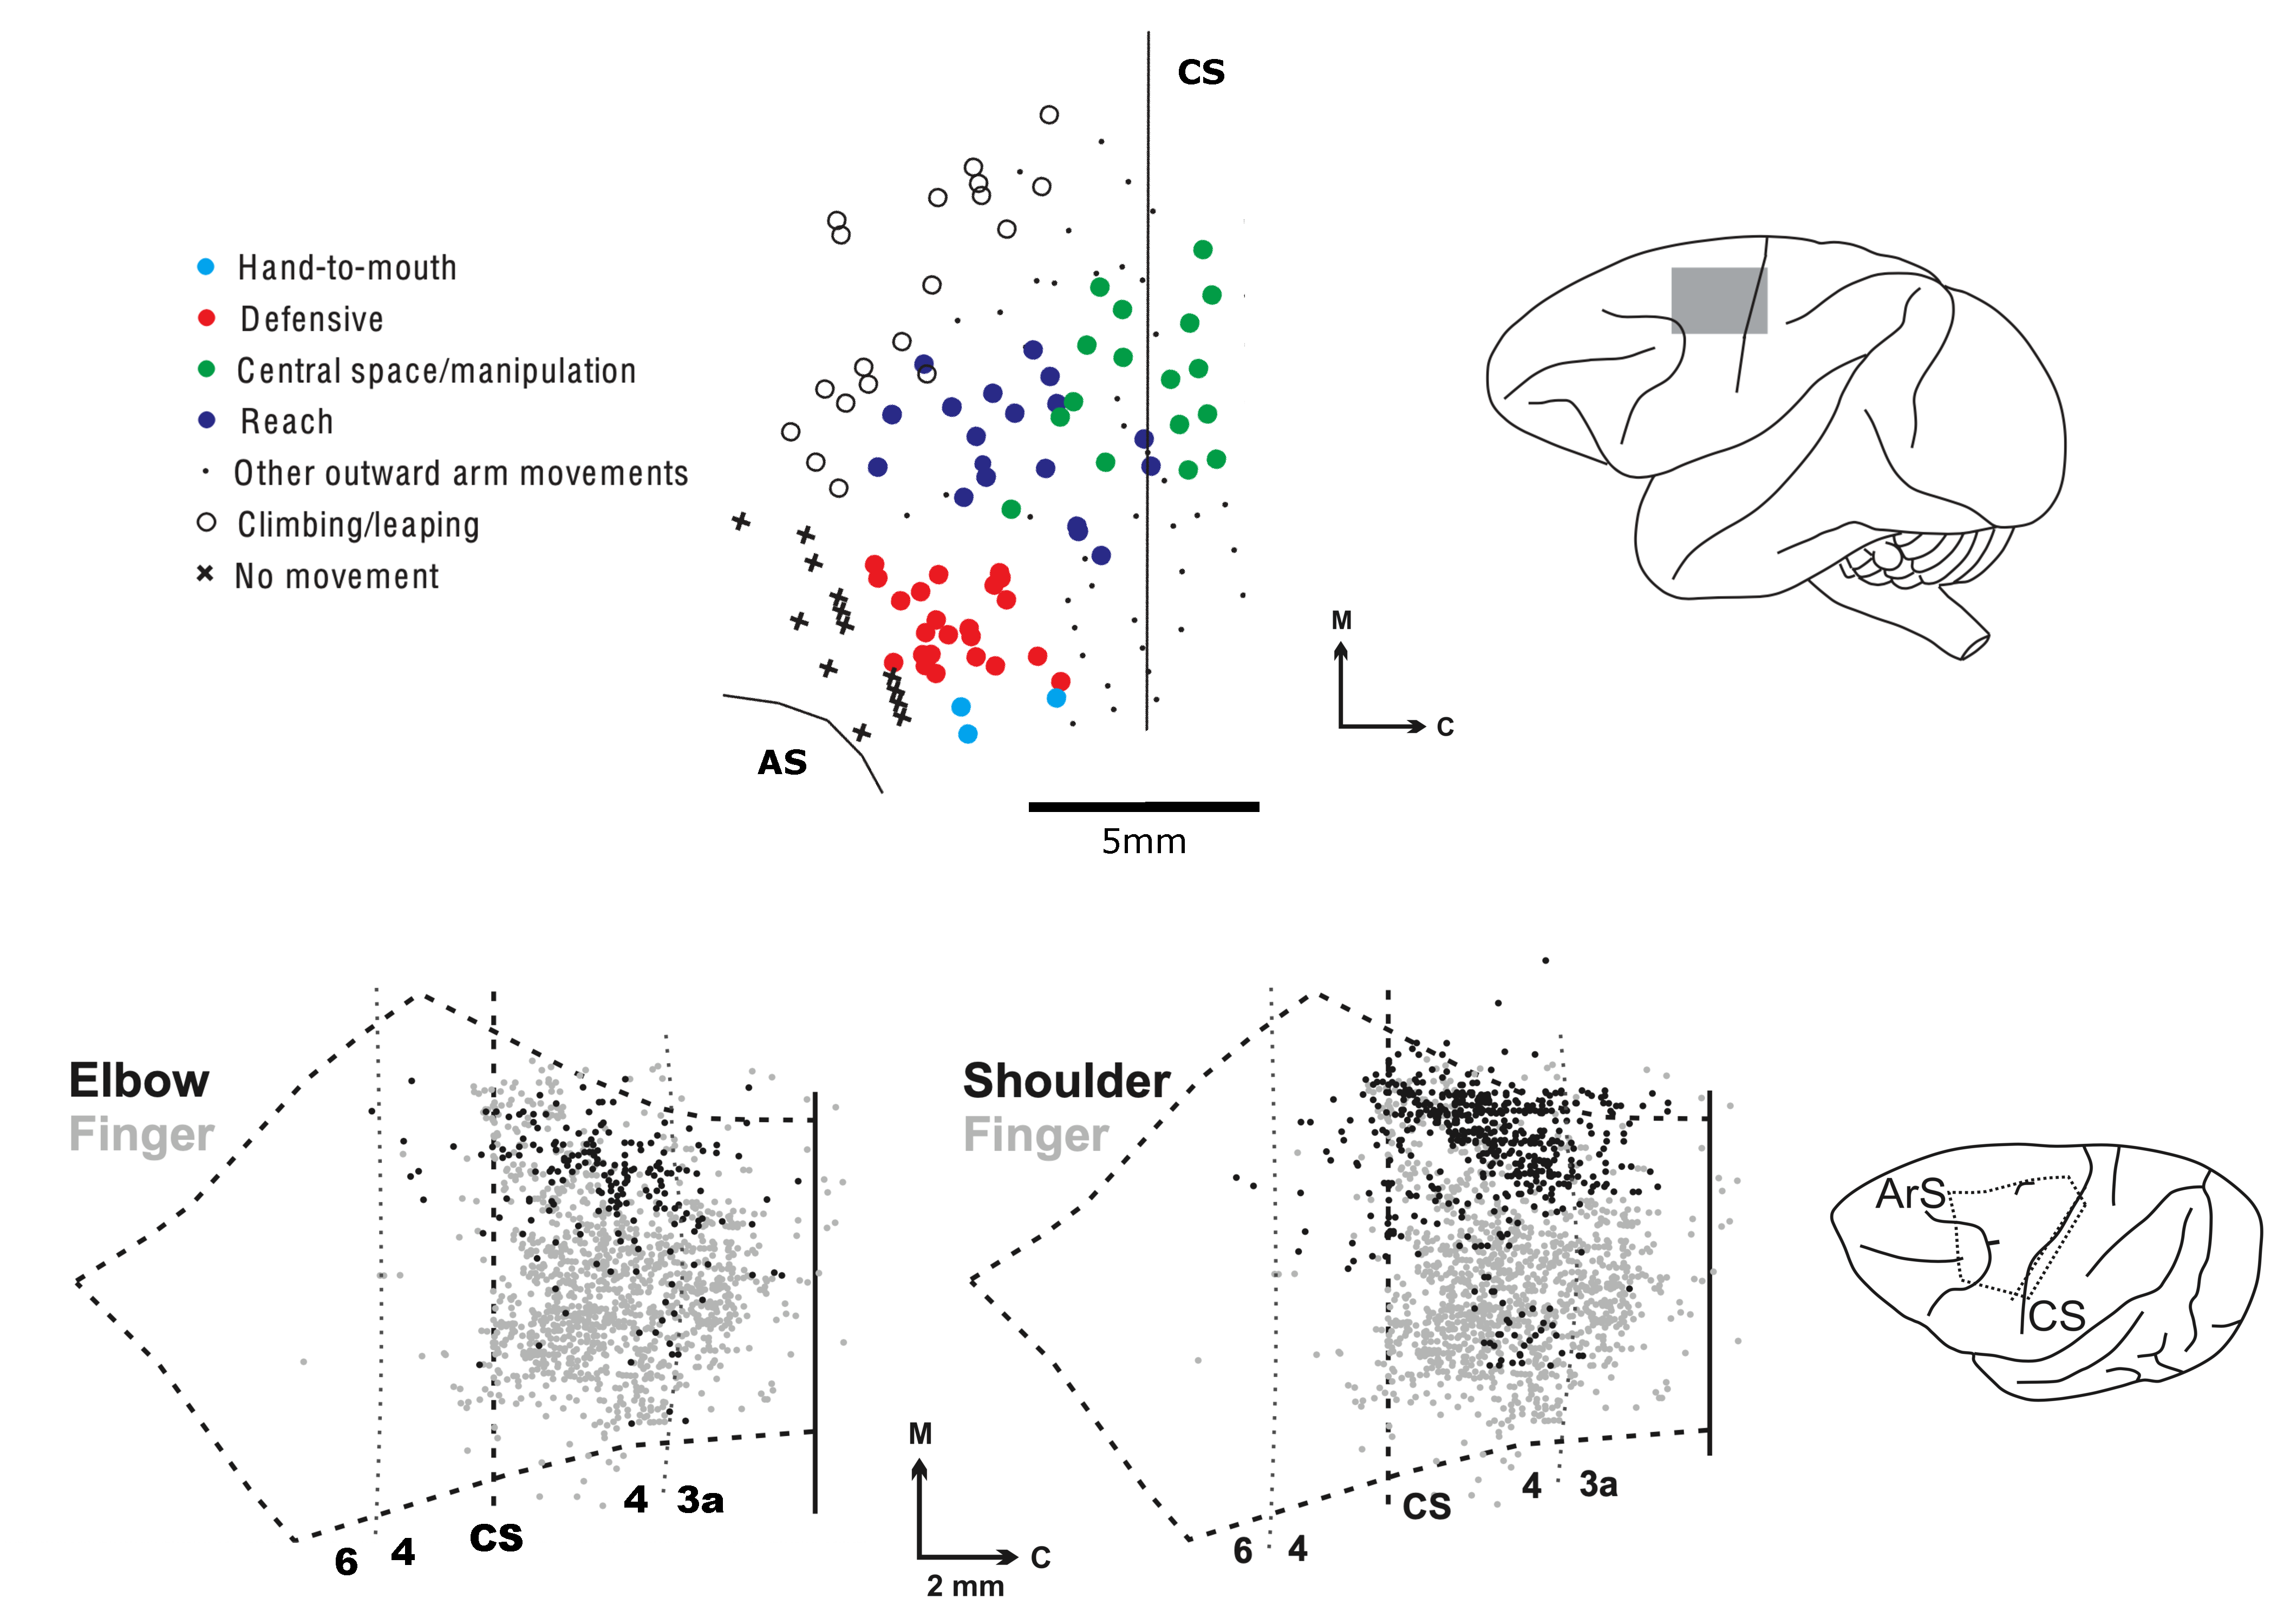
\includegraphics[width=1.0\textwidth]{background_theory/strick_graziano.pdf}
  \caption[Comparing the work of Strick and Graziano]{Similarities between electrical stimulation on behavorial timescales and rabies tracing identification of CM cells. CM cells are largely confined to the caudal half of M1, while this region tends to evoke complex manipulatory movements when electrically stimulated. (Top Left) Corticomotoneuronal (CM) cells traced using rabies from muscles of the elbow and finger. (Top Right) CM cells traced using rabies from muscles of the shoulder and finger. (Bottom) Complex movements evoked by 500ms electrical stimulation pulse trains. Adapted from Graziano 2005 and Rathelot et al.~2009{[}@graziano2005;@Rathelot2009{]}.}\label{fig:strick_graziano}
\end{figure}

Graziano writes:

\begin{quote} 
  ``The usefulness of a feedback-dependent mapping from cortex to muscles is that it can in principle allow neurons in motor cortex to control a diversity of movement variables, such as direction, speed, hand position, or posture that transcend a fixed pattern of muscle activation. If the network receives feedback information about a specific movement variable, then it can learn to control that variable.''
\end{quote}

Muscle activity is, in this sense, a readout from a network transforming state-dependent inputs into movement goals. Rather than choosing muscle patterns in reconfigurable blocks, it creatively constructs and sculpts movement. The hierarchy of the motor system may not be rigidly organized around a particular set of variables. As shown in \{+@fig:motor\_system\}, many loops exist connecting cortex with the spinal cord, the cerebellum, the basal ganglia, and the sensorimotor periphery. Each of these loops contributes information for the flexible activation of the relevant action maps. Put simply, prevailing evidence suggests that cerebellar loops provide predictive state information while basal gangliar loops provide state and/or action value information. Taken together, this work provides an image of the incredible complexity which generates dexterous movements of the hand. This is the foundation on which we can work to build experiments which elucidate the computations involved in the production of skilled movement. We aim to connect our results back to what is known about the system we are attempting to reverse-engineer in order to inspire future inquiries into the inner workings of the movement machine.

\begin{figure}[H]
\centering
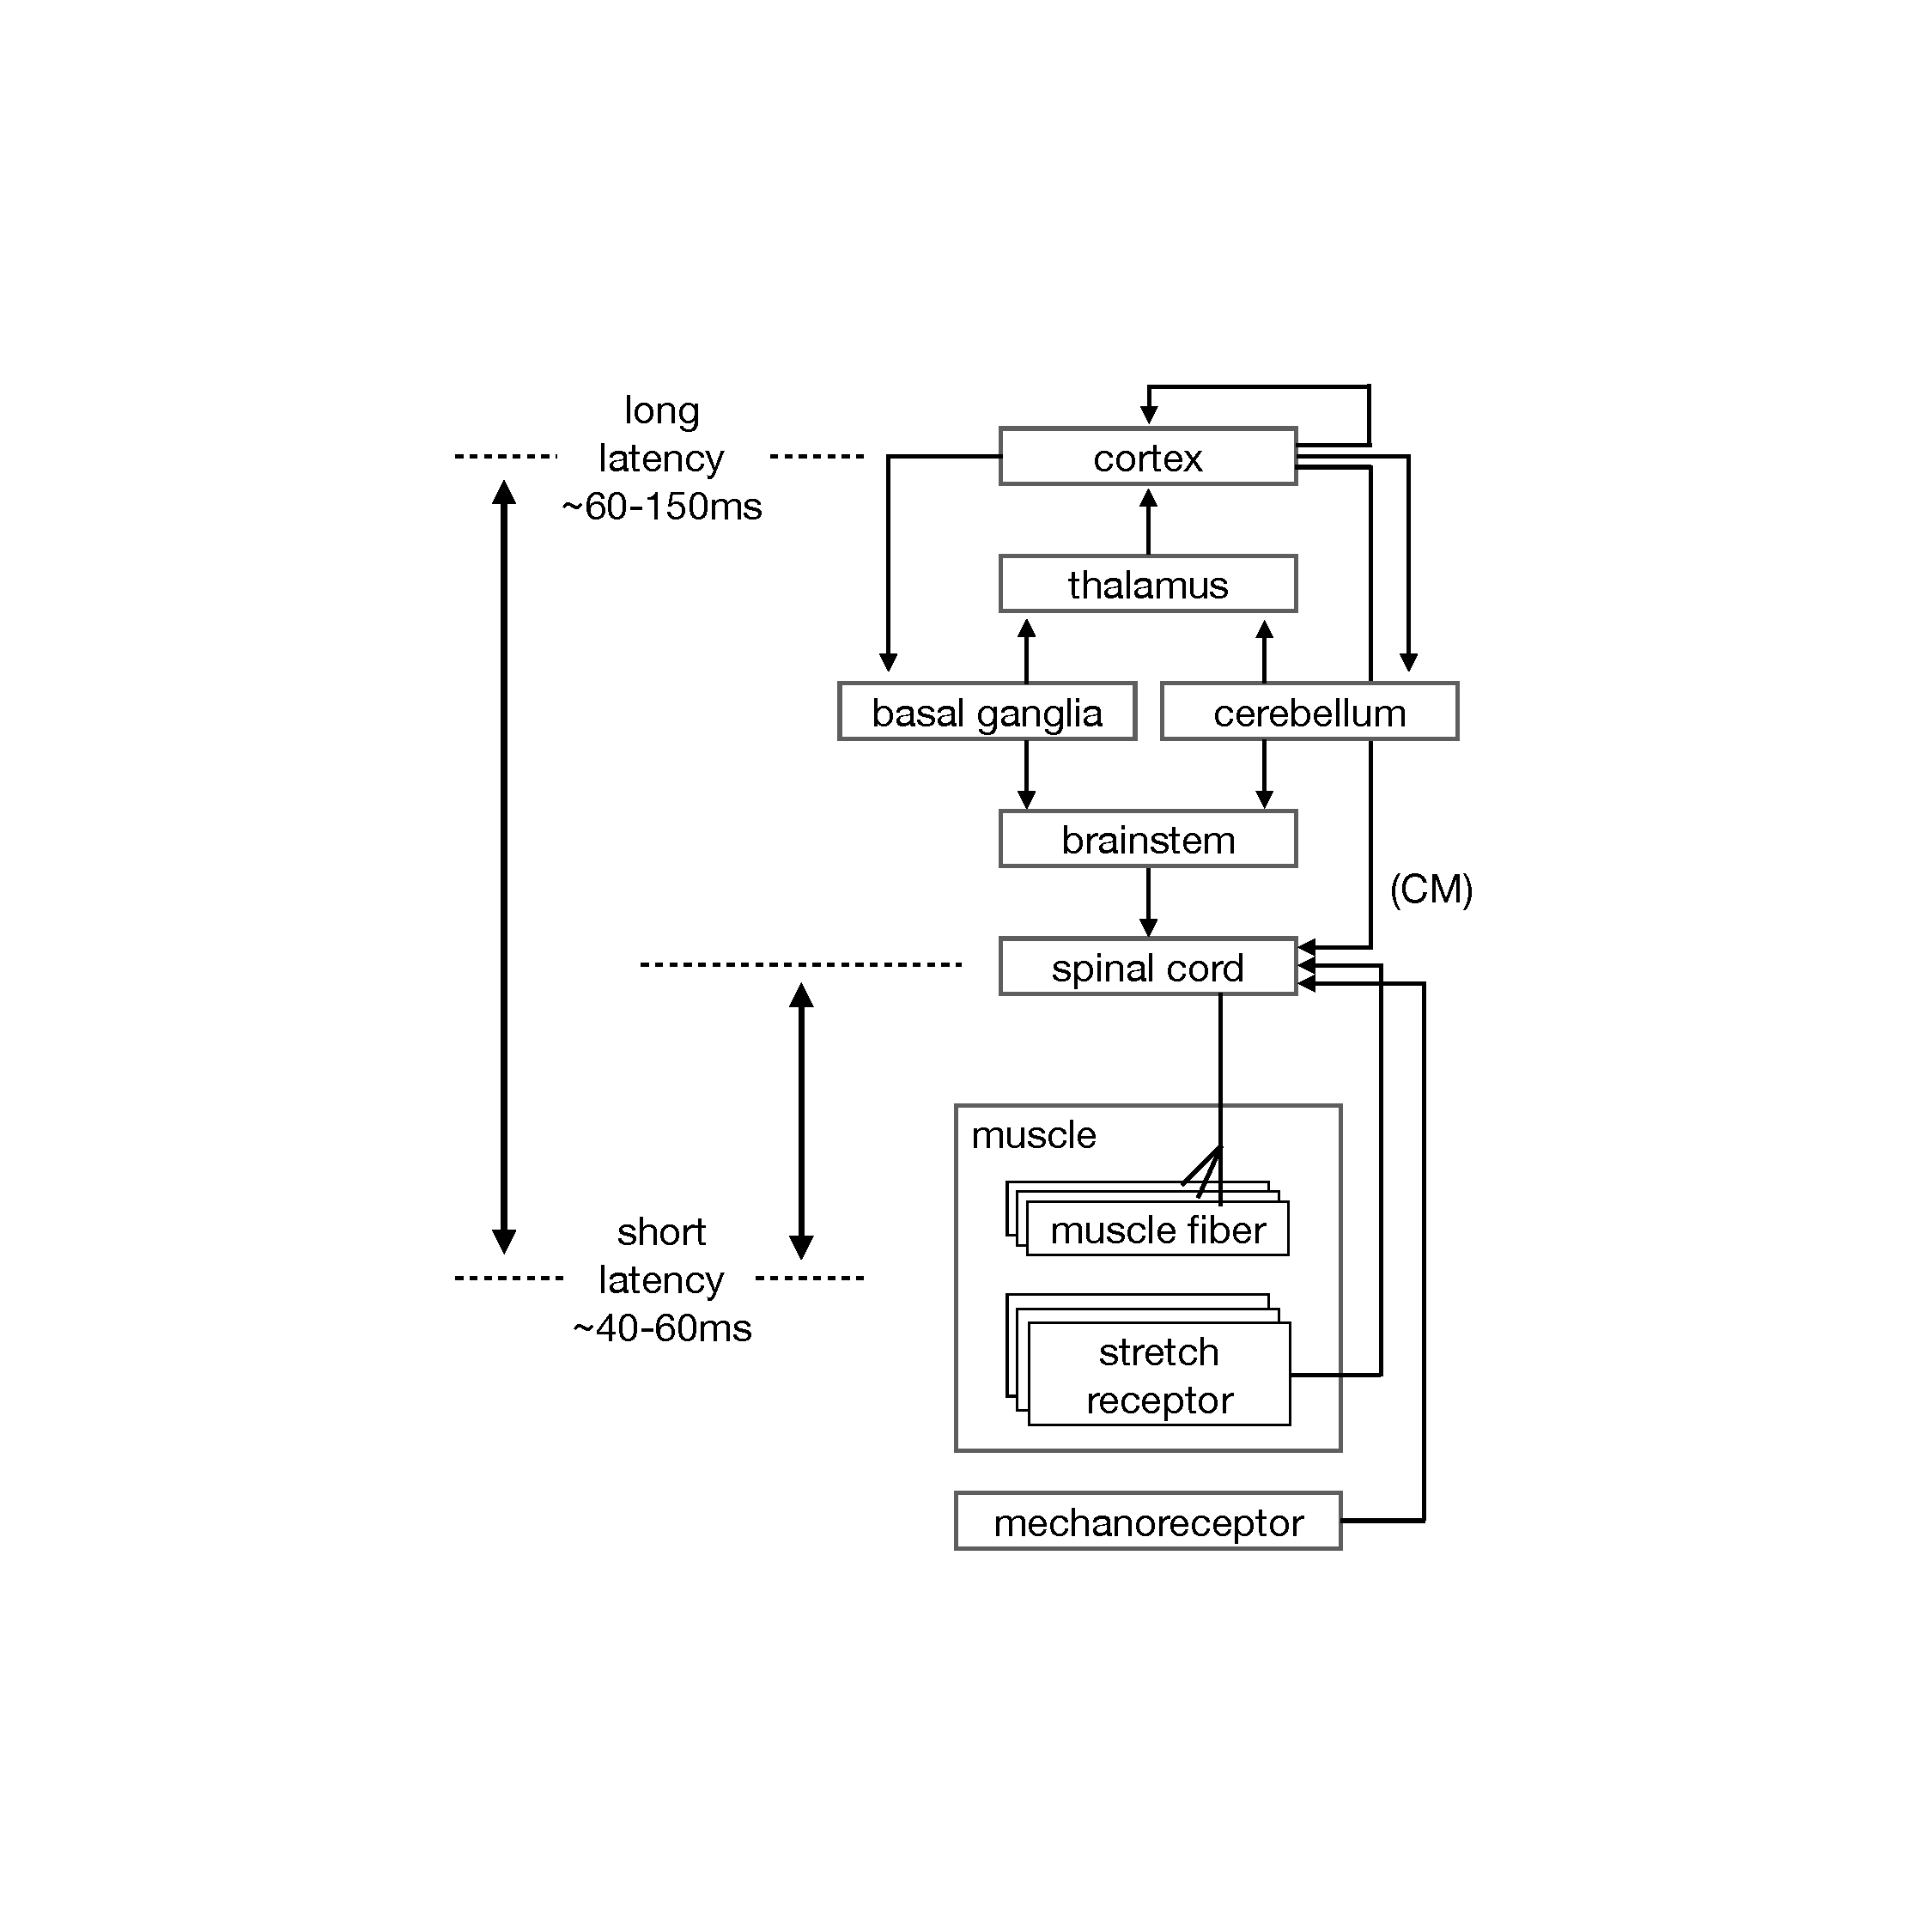
\includegraphics[width=1.0\textwidth]{background_theory/motor_system.pdf}
\caption[Motor sytem schematic]{Overview sketch of the motor system depicting the the redundancy of the system both hierarchically (multiple muscle fibers are innervated by the same motor neuron, many motor neurons innervate the same muscle) as well as heterarchically (parallel spinal, corticomotoneuronal, cerebellum, basal gangliar feedback loops). Parallel reflex responses can be classified as long latency (approximately 60-150ms) and short latency (approximately 60ms). We hope to consider the parallelism and redundancy of the motor system to inspire our data analyses and models of motor computation.}\label{fig:motor_system}
\end{figure}


  




\cleardoublepage\printendnotes%
\ifSubfilesClassLoaded{%
    \newpage%
    \bibliography{../bib/bibliography}%
}{}%
\end{document}
